
\documentclass[11pt]{article}
\usepackage[a4paper,margin=1in]{geometry}
\usepackage{amsmath,amssymb}
\usepackage{graphicx}
\usepackage[dvipsnames]{xcolor}
\usepackage{hyperref}
\usepackage{enumitem}
\usepackage{tabularx}
\usepackage{longtable}
\usepackage{booktabs}
\usepackage[most]{tcolorbox}
\usepackage{titlesec}
\usepackage{xurl}
\usepackage{fancyhdr}
\usepackage{setspace}
\usepackage{tikz}
\usetikzlibrary{positioning,arrows.meta}
\usepackage[T1]{fontenc}
\usepackage{lmodern}
\setlength{\parindent}{0pt}
\setlength{\parskip}{8pt}
\setlength{\headheight}{14pt}
\setstretch{1.12}
\setlist[itemize]{leftmargin=1.5em, nosep}
\setlist[enumerate]{leftmargin=1.5em, nosep}
\providecommand{\tightlist}{\setlength{\itemsep}{0pt}\setlength{\parskip}{0pt}}
\hypersetup{colorlinks=true,linkcolor=MidnightBlue,urlcolor=MidnightBlue}
\pagestyle{fancy}
\fancyhf{}
\rhead{\thepage}
\renewcommand{\headrulewidth}{0pt}
\renewcommand{\footrulewidth}{0pt}
\titleformat{\section}{\Large\bfseries\color{MidnightBlue}}{\thesection}{0.6em}{}
\titleformat{\subsection}{\bfseries}{}{0em}{}


\begin{document}

\begin{center}\LARGE\bfseries Bayesian Networks for Uncertain Agent Reasoning\end{center}

\begin{center}\large Block 4 Day 1\end{center}

\begin{tcolorbox}[colback=MidnightBlue!4,colframe=MidnightBlue,title={Session Overview},fonttitle=\bfseries,breakable]
\textbf{Session objective:} Build Bayesian networks that express uncertain structure clearly and reason about dependence using concrete scenarios rather than only abstract symbols.

\textbf{Timing target (min):} 70

\textbf{Topic anchors:} bayesian networks; conditional independence; d-separation; healthcare; autonomous driving; financial risk

\textbf{Padlet board:} \url{https://padlet.com/qmul/b4-d1-u2uhk8999arw5i4z}
\end{tcolorbox}

\section*{Exercises}

\begin{tcolorbox}[colback=white,colframe=MidnightBlue,title={Q1 Starter Intuition},fonttitle=\bfseries,breakable]
\begin{center}
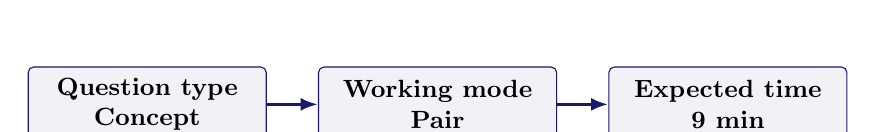
\begin{tikzpicture}[
node distance=0.65cm,
box/.style={draw=MidnightBlue, rounded corners=2pt, minimum height=0.95cm, align=center, font=\small\bfseries, fill=MidnightBlue!6, text width=0.23\linewidth},
arrow/.style={-{Latex[length=2.2mm]}, very thick, MidnightBlue}
]
\node[box] (type) {Question type\\Concept};
\node[box, right=of type] (mode) {Working mode\\Pair};
\node[box, right=of mode] (time) {Expected time\\9 min};
\draw[arrow] (type) -- (mode);
\draw[arrow] (mode) -- (time);
\end{tikzpicture}
\end{center}

{\large\bfseries\color{MidnightBlue} Prompt}\par\medskip
A Bayesian network has a directed graph and conditional probability tables. In simple language, explain what the graph tells us, what the tables tell us, and why we need both parts together. Use one small example from healthcare, driving, or daily life.

{\large\bfseries\color{MidnightBlue} Task details}\par\medskip
\begin{itemize}\item \textbf{Type:} concept
\item \textbf{Mode:} pair
\item \textbf{Time:} 9 min
\item \textbf{Deliverable:} short explanation
\item \textbf{Assessment focus:} explain what information the graph gives and what information the probabilities give
\item \textbf{Expected length:} 3 bullets + 1 example\end{itemize}

{\large\bfseries\color{MidnightBlue} How to submit}\par\medskip
Post one pair Padlet comment with three short bullets and one example.

{\large\bfseries\color{MidnightBlue} Discussion in class}\par\medskip
If you had to build one part first in practice, which part would it be?

{\large\bfseries\color{MidnightBlue} Why this helps}\par\medskip
Useful for theory questions that ask what a Bayesian network contains and why the structure and numbers are both needed.

{\large\bfseries\color{MidnightBlue} References}\par\medskip
\begin{itemize}\item Russell \& Norvig (2021) AIMA 4e, Ch.12-13, pp.385-460
\item Poole \& Mackworth (2023) 3e, Ch.9, pp.375-458\end{itemize}
\end{tcolorbox}

\begin{tcolorbox}[colback=white,colframe=MidnightBlue,title={Q2 Structured Problem},fonttitle=\bfseries,breakable]
\begin{center}
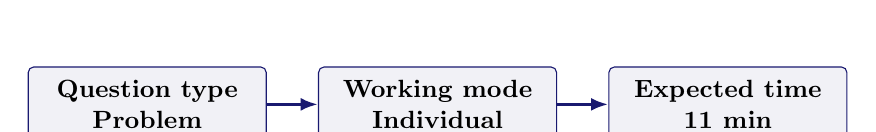
\begin{tikzpicture}[
node distance=0.65cm,
box/.style={draw=MidnightBlue, rounded corners=2pt, minimum height=0.95cm, align=center, font=\small\bfseries, fill=MidnightBlue!6, text width=0.23\linewidth},
arrow/.style={-{Latex[length=2.2mm]}, very thick, MidnightBlue}
]
\node[box] (type) {Question type\\Problem};
\node[box, right=of type] (mode) {Working mode\\Individual};
\node[box, right=of mode] (time) {Expected time\\11 min};
\draw[arrow] (type) -- (mode);
\draw[arrow] (mode) -- (time);
\end{tikzpicture}
\end{center}

{\large\bfseries\color{MidnightBlue} Prompt}\par\medskip
Consider three small patterns using named variables instead of A, B, and C. (1) Rain -\textgreater{} WetRoad -\textgreater{} TrafficDelay, (2) BatteryLow \textless- OldDevice -\textgreater{} SlowPerformance, (3) Infection -\textgreater{} Fever \textless- Exercise. For each pattern, decide whether the two end variables are dependent when nothing is observed and when the middle variable is observed.

{\large\bfseries\color{MidnightBlue} Task details}\par\medskip
\begin{itemize}\item \textbf{Type:} problem
\item \textbf{Mode:} individual
\item \textbf{Time:} 11 min
\item \textbf{Deliverable:} dependence judgements
\item \textbf{Assessment focus:} reason about dependence and independence using named scenario variables
\item \textbf{Expected length:} 6 answers + short reasons\end{itemize}

{\large\bfseries\color{MidnightBlue} How to submit}\par\medskip
Post your own Padlet comment with six dependence or independence decisions and one short reason for each.

{\large\bfseries\color{MidnightBlue} Discussion in class}\par\medskip
Which pattern changes most when you observe the middle variable?

{\large\bfseries\color{MidnightBlue} Why this helps}\par\medskip
Direct practice for conditional-independence reasoning without copying the abstract exam pattern exactly.

{\large\bfseries\color{MidnightBlue} References}\par\medskip
\begin{itemize}\item Russell \& Norvig (2021) AIMA 4e, Ch.12-13, pp.385-460
\item Poole \& Mackworth (2023) 3e, Ch.9, pp.375-458\end{itemize}
\end{tcolorbox}

\begin{tcolorbox}[colback=white,colframe=MidnightBlue,title={Q3 Structured Problem},fonttitle=\bfseries,breakable]
\begin{center}
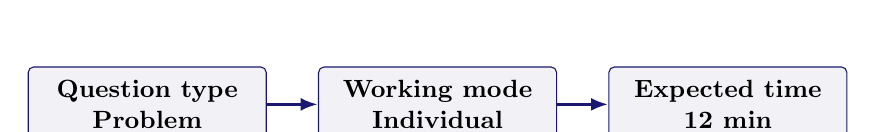
\begin{tikzpicture}[
node distance=0.65cm,
box/.style={draw=MidnightBlue, rounded corners=2pt, minimum height=0.95cm, align=center, font=\small\bfseries, fill=MidnightBlue!6, text width=0.23\linewidth},
arrow/.style={-{Latex[length=2.2mm]}, very thick, MidnightBlue}
]
\node[box] (type) {Question type\\Problem};
\node[box, right=of type] (mode) {Working mode\\Individual};
\node[box, right=of mode] (time) {Expected time\\12 min};
\draw[arrow] (type) -- (mode);
\draw[arrow] (mode) -- (time);
\end{tikzpicture}
\end{center}

{\large\bfseries\color{MidnightBlue} Prompt}\par\medskip
A student is deciding whether to cycle to campus. Build a small Bayesian network with at least five nodes using some of these ideas: weather, bike condition, traffic, lateness risk, mood, and final choice. Identify which variable is hidden or uncertain in the most useful way and explain why.

{\large\bfseries\color{MidnightBlue} Task details}\par\medskip
\begin{itemize}\item \textbf{Type:} problem
\item \textbf{Mode:} individual
\item \textbf{Time:} 12 min
\item \textbf{Deliverable:} local BN design
\item \textbf{Assessment focus:} choose nodes, edges, and one hidden variable for a compact BN
\item \textbf{Expected length:} 5 nodes + 5 edges + 1 note\end{itemize}

{\large\bfseries\color{MidnightBlue} How to submit}\par\medskip
Post your own Padlet comment with the node list, edge list, and one short note on the most important hidden variable.

{\large\bfseries\color{MidnightBlue} Discussion in class}\par\medskip
Which edge in your network would be hardest to justify causally?

{\large\bfseries\color{MidnightBlue} Why this helps}\par\medskip
Supports case questions where students must design a network instead of only reading one.

{\large\bfseries\color{MidnightBlue} References}\par\medskip
\begin{itemize}\item Russell \& Norvig (2021) AIMA 4e, Ch.12-13, pp.385-460
\item Poole \& Mackworth (2023) 3e, Ch.9, pp.375-458\end{itemize}
\end{tcolorbox}

\begin{tcolorbox}[colback=white,colframe=MidnightBlue,title={Q4 Collaborative Mini-Case},fonttitle=\bfseries,breakable]
\begin{center}
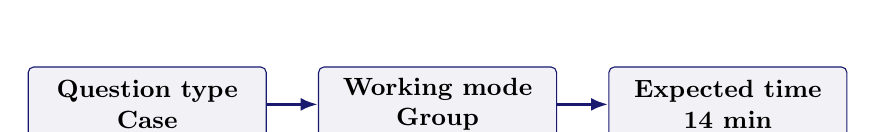
\begin{tikzpicture}[
node distance=0.65cm,
box/.style={draw=MidnightBlue, rounded corners=2pt, minimum height=0.95cm, align=center, font=\small\bfseries, fill=MidnightBlue!6, text width=0.23\linewidth},
arrow/.style={-{Latex[length=2.2mm]}, very thick, MidnightBlue}
]
\node[box] (type) {Question type\\Case};
\node[box, right=of type] (mode) {Working mode\\Group};
\node[box, right=of mode] (time) {Expected time\\14 min};
\draw[arrow] (type) -- (mode);
\draw[arrow] (mode) -- (time);
\end{tikzpicture}
\end{center}

{\large\bfseries\color{MidnightBlue} Prompt}\par\medskip
Start from your group's BN design in a domain such as healthcare triage, autonomous driving risk, or financial risk. Pick one child node with two or three parents and sketch a small local conditional probability table. You do not need every number in the full network, only one local CPT and the reasoning behind the values.

{\large\bfseries\color{MidnightBlue} Task details}\par\medskip
\begin{itemize}\item \textbf{Type:} case
\item \textbf{Mode:} group
\item \textbf{Time:} 14 min
\item \textbf{Deliverable:} CPT sketch
\item \textbf{Assessment focus:} move from graph structure to simple probability design
\item \textbf{Expected length:} 1 local CPT + 3 justification bullets\end{itemize}

{\large\bfseries\color{MidnightBlue} How to submit}\par\medskip
Post one group Padlet comment with the chosen node, the local CPT sketch, and three bullets explaining the probabilities.

{\large\bfseries\color{MidnightBlue} Discussion in class}\par\medskip
Which parent has the strongest effect on the child node in your CPT?

{\large\bfseries\color{MidnightBlue} Why this helps}\par\medskip
Useful for questions that move from structure to parameterisation without turning into a full arithmetic problem.

{\large\bfseries\color{MidnightBlue} References}\par\medskip
\begin{itemize}\item Russell \& Norvig (2021) AIMA 4e, Ch.12-13, pp.385-460
\item Poole \& Mackworth (2023) 3e, Ch.9, pp.375-458\end{itemize}
\end{tcolorbox}

\begin{tcolorbox}[colback=white,colframe=MidnightBlue,title={Q5 Exam-Style Constructed Response},fonttitle=\bfseries,breakable]
\begin{center}
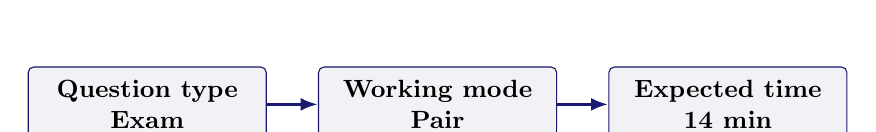
\begin{tikzpicture}[
node distance=0.65cm,
box/.style={draw=MidnightBlue, rounded corners=2pt, minimum height=0.95cm, align=center, font=\small\bfseries, fill=MidnightBlue!6, text width=0.23\linewidth},
arrow/.style={-{Latex[length=2.2mm]}, very thick, MidnightBlue}
]
\node[box] (type) {Question type\\Exam};
\node[box, right=of type] (mode) {Working mode\\Pair};
\node[box, right=of mode] (time) {Expected time\\14 min};
\draw[arrow] (type) -- (mode);
\draw[arrow] (mode) -- (time);
\end{tikzpicture}
\end{center}

{\large\bfseries\color{MidnightBlue} Prompt}\par\medskip
Choose one assumption in your Bayesian network design, such as a missing hidden cause, a questionable edge, or an unrealistic conditional-independence claim. Explain how that assumption could distort inference and what you would change to improve the model.

{\large\bfseries\color{MidnightBlue} Task details}\par\medskip
\begin{itemize}\item \textbf{Type:} exam
\item \textbf{Mode:} pair
\item \textbf{Time:} 14 min
\item \textbf{Deliverable:} structured response
\item \textbf{Assessment focus:} analyse one weak modelling assumption and its effect on inference
\item \textbf{Expected length:} 180-230 words\end{itemize}

{\large\bfseries\color{MidnightBlue} How to submit}\par\medskip
Post one pair Padlet comment with the assumption, the failure it causes, and one repair.

{\large\bfseries\color{MidnightBlue} Discussion in class}\par\medskip
Is a missing hidden variable usually more damaging than one wrong probability entry?

{\large\bfseries\color{MidnightBlue} Why this helps}\par\medskip
Strengthens reasoning about model assumptions in a new setting.

{\large\bfseries\color{MidnightBlue} References}\par\medskip
\begin{itemize}\item Russell \& Norvig (2021) AIMA 4e, Ch.12-13, pp.385-460
\item Poole \& Mackworth (2023) 3e, Ch.9, pp.375-458\end{itemize}
\end{tcolorbox}

\begin{tcolorbox}[colback=white,colframe=MidnightBlue,title={Q6 Stretch Extension},fonttitle=\bfseries,breakable]
\begin{center}
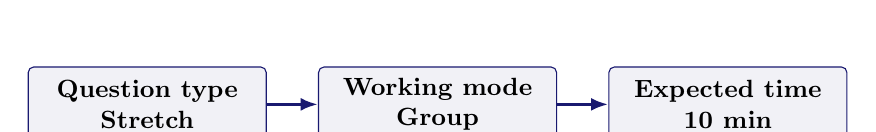
\begin{tikzpicture}[
node distance=0.65cm,
box/.style={draw=MidnightBlue, rounded corners=2pt, minimum height=0.95cm, align=center, font=\small\bfseries, fill=MidnightBlue!6, text width=0.23\linewidth},
arrow/.style={-{Latex[length=2.2mm]}, very thick, MidnightBlue}
]
\node[box] (type) {Question type\\Stretch};
\node[box, right=of type] (mode) {Working mode\\Group};
\node[box, right=of mode] (time) {Expected time\\10 min};
\draw[arrow] (type) -- (mode);
\draw[arrow] (mode) -- (time);
\end{tikzpicture}
\end{center}

{\large\bfseries\color{MidnightBlue} Prompt}\par\medskip
Suppose you have only a small amount of data for your domain. Propose a short process for estimating the missing conditional probabilities using expert knowledge, sparse observations, and one conflict-resolution rule when they disagree.

{\large\bfseries\color{MidnightBlue} Task details}\par\medskip
\begin{itemize}\item \textbf{Type:} stretch
\item \textbf{Mode:} group
\item \textbf{Time:} 10 min
\item \textbf{Deliverable:} elicitation protocol
\item \textbf{Assessment focus:} connect expert judgement and sparse data to BN parameter design
\item \textbf{Expected length:} 5 steps\end{itemize}

{\large\bfseries\color{MidnightBlue} How to submit}\par\medskip
Post one group Padlet comment with a five-step elicitation process.

{\large\bfseries\color{MidnightBlue} Discussion in class}\par\medskip
When should the data be allowed to override expert opinion?

{\large\bfseries\color{MidnightBlue} Why this helps}\par\medskip
Good extension for applied questions on how uncertain models are built in practice.

{\large\bfseries\color{MidnightBlue} References}\par\medskip
\begin{itemize}\item Russell \& Norvig (2021) AIMA 4e, Ch.12-13, pp.385-460
\item Poole \& Mackworth (2023) 3e, Ch.9, pp.375-458\end{itemize}
\end{tcolorbox}

\section*{Submission Instructions}

Use the seeded Padlet posts for Q1--Q6. Q2 and Q3 are individual. Q1 and Q5 are pair tasks. Q4 and Q6 should be one joint group comment. Start each comment with your names or group label.

\section*{Whole-Class Debrief Prompts}

\begin{itemize}
\tightlist
\item
  Which BN edge was easiest to justify, and which one was hardest?
\item
  Which scenario pattern made dependence feel most intuitive?
\item
  When does a weak BN assumption matter more than slightly inaccurate probability numbers?
\end{itemize}

\section*{Exam Transfer Note (Day-Level)}

Maps to exam questions on BN structure, dependence and independence, local CPT design, and assumption analysis.

\end{document}
